\chapter{Grundlagen der GPU-Programmierung}

Um die in dieser Arbeit vorgestellten Herausforderungen bei der Verarbeitung von String-Daten mit Grafikprozessoren, nachfolgend auch GPU genannt, verstehen zu können, ist zunächst ein Verständnis der grundlegenden Eigenschaften aktueller Hardware nötig.
Dabei beschränkt sich diese Untersuchung auf die Grafikkarten-Serie Maxwell von NVIDIA, die hier besprochenen Prinzipien lassen sich allerdings auch auf andere GPU anderer Hersteller übertragen und finden dort ebenfalls Anwendung.

\section{Grundaufbau einer NVIDIA-Grafikkarte}

Der Hauptprozessor eines Computers, auch \emph{Central Processing Unit (CPU)} genannt, arbeitet eher sequenziell schwerwiegende Threads ab, wodurch individuelle Operationen schnell abgearbeitet werden können, ein hoher Durchsatz allerdings schwierig zu erreichen ist.
Für die Verarbeitung großer Datenmengen wurden daher spezielle Co-Prozessoren in Form von Grafikkarten entwickelt, die hochgradig parallel arbeiten und somit einen massiven Durchsatz erreichen können.
Die \emph{Graphics Processing Unit (GPU)} bildet das Herzstück der Grafikkarte.
Sie besteht aus einer hohen Anzahl an Kernen, die zwar individuell eine vergleichsweise geringe Leistung besitzen, allerdings aufgrund ihrer hohen Anzahl in datenparallelen Anwendungsfällen in Kombination mit einer hohen Speicherbandbreite eine hervorragende Performanz bieten.

Neben der GPU benötigt eine Grafikkarte noch weitere Peripherie, um effizient funktionieren zu können.
Zur Speicherung der zu verarbeitenden Daten gibt es eigenständige Speichermodule, die unabhängig vom Hauptspeicher des Computers verwaltet werden.
Für die NVIDIA GTX950, welche im Folgenden als Beispiel genutzt werden soll, beträgt die Größe dieses Speichers 2 GB.
Über eine PCI-Express-Anbindung wird die Kommunikation mit dem Hauptprozessor und die Übertragung der Daten zwischen den Speicherbereichen realisiert.

\begin{figure}[ht]
	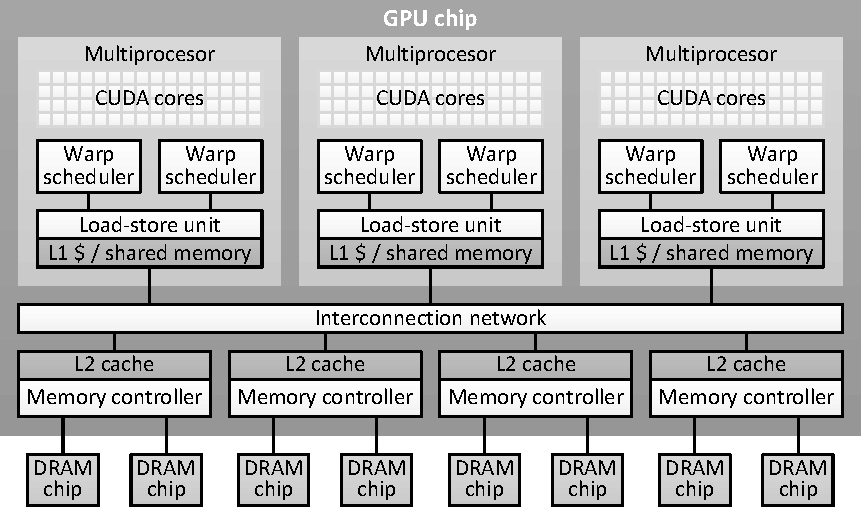
\includegraphics[]{bilder/gpu_architecture.pdf}
	\caption{Architektur einer GPU \cite{Volkov2016}}
	\label{gpu_architecture}
\end{figure}

Wie in Abbildung \ref{gpu_architecture} dargestellt, lässt sich die GPU wiederum in kleinere Module, sogenannte \emph{Streaming Multiprocessors (SM)}, unterteilen, welche jeweils eigenständige Recheneinheiten darstellen.
Eine GTX950 besitzt beispielsweise sechs dieser Streaming Multiprocessors, welche sich ebenfalls in kleinere Einheiten unterteilen lassen.
Die SM bestehen aus vier unabhängigen Blöcken von Rechenkernen, welche jeweils 32 skalare Recheneinheiten, auch \emph{CUDA-Kerne} genannt, beinhalten.
Jeder dieser Blöcke besitzt einen eigenen Scheduler und einige Unterstützungselektronik, sodass diese logisch gesehen ebenfalls unabhängig voneinander arbeiten können. \cite{Nvidia2014}
Bei sechs Streaming Multiprocessors mit jeweils vier Blöcken und 32 Recheneinheiten pro Block besitzt die GTX950 also 768 Kerne, welche über eine Programmierschnittstelle angesprochen werden können.

\section{Scheduling auf GPU}

Um die hohe Anzahl von Kernen innerhalb einer GPU effizient mit Arbeit versorgen zu können, wird schnell klar, dass ein individuelles Scheduling für die einzelnen Recheneinheiten durch den großen Overhead unpraktikabel wäre.
Aus diesem Grund werden die Threads eines Programms in sogenannte \emph{Warps} zusammengefasst, was damit die kleinste Einheit für das Scheduling bildet.
Ein Warp enthält dabei genau 32 Threads, welche in diesem Kontext auch \emph{Lanes} genannt werden.
Mehrere Warps werden außerdem zu \emph{Blöcken} zusammengefasst, welche schließlich als Ganzes an einzelne Streaming Multiprocessors zugewiesen werden.
Innerhalb eines SM werden Warps ausgetauscht, wenn der vorher aktive Warp beispielsweise auf einen Speicherzugriff wartet, um die dadurch entstehende Latenz zu verstecken.

Über die Anzahl der Threads pro Block und die gesamte Anzahl der Blöcke, ist die Konfiguration des sogenannten \emph{Grids} definiert.
Die Grid-Konfiguration nimmt starken Einfluss auf die Ausführungszeit der Software.
Beispielsweise kann eine zu geringe Anzahl von Threads pro Block dazu führen, dass eventuell entstehende Latenzen nicht mehr so gut versteckt werden können, da nicht genug Threads innerhalb eines SM vorhanden sind.
Eine zu hohe Anzahl von Threads pro Block kann allerdings auch von Nachteil sein, da Hardwareressourcen wie die Speichergröße pro SM gegebenenfalls nicht mehr ausreichen und das Programm nicht mehr korrekt funktioniert.
Das Finden der richtigen Parameter gestaltet sich als äußerst schwierig, da die verwendete Hardware ein komplexes Konstrukt mit vielen Faktoren bildet, die auf unterschiedliche Aspekte des Grids Einfluss nehmen.

Eine für die Programmierung von GPU entscheidende Eigenschaft besteht darin, dass die Threads innerhalb eines Warps parallel ausgeführt werden.
Ähnlich wie bei dem Prinzip \emph{Single Instruction Multiple Data (SIMD)}, führen die Threads in einem Warp die Instruktionen synchron aus, sodass dieses Prinzip auch \emph{Single Instruction Multiple Threads (SIMT)} genannt wird.
Die Trennung in mehrere Threads, bietet hierbei den Vorteil, dass eigene Register angesprochen werden können, an unterschiedlichen Stellen im Speicher gelesen werden kann und Threads verschiedene Kontrollflüsse verfolgen können.
Prozesse laufen außerdem zwar logisch parallel ab, allerdings muss dies nicht notwendigerweise physikalisch auch so sein, sodass in einigen Fällen eine höhere Leistung erzielt werden kann.
Für die optimale Performanz einzelner Operationen sollte allerdings gewährleistet sein, dass die Threads größtenteils synchron ausgeführt werden.

Bei der Verwendung von Branching-Instruktionen kann es vorkommen, dass unterschiedliche Threads verschiedene Kontrollflüsse durchlaufen, was auch als \emph{Divergenz} bezeichnet wird.
Da allerdings alle Threads identische Instruktionen ausführen müssen, führt dies dazu, dass sämtliche Threads in einem Warp alle notwendigen Kontrollflüsse durchlaufen und dabei gegebenenfalls das Ergebnis verwerfen, wenn diese sich logisch gesehen in einem anderen Zweig befinden.
Alle Threads, für die der aktuell bearbeitete Kontrollfluss nicht relevant ist, werden als inaktiv bezeichnet.
Inaktive Threads warten somit lediglich auf die aktiven Threads, bis diese die Arbeit innerhalb ihres Kontrollflusses abgeschlossen haben, sodass an dieser Stelle gegebenenfalls massiv Rechenleistung verschwendet wird.
In dieser Problematik liegt der Grund dafür, dass die Verarbeitung von Strings auf Grafikkarten aufgrund ihrer variablen Länge problematisch ist, da die auftretenden Kontrollflüsse divergieren.

\section{Synchronisation von Threads}
\label{sec:synchronisation_von_threads}

Der Compiler und die GPU selbst versuchen innerhalb eines Warps die Anzahl der synchron ausgeführten Operationen zu maximieren, da dadurch eine höhere Leistung erzielt wird. \cite{Nickolls2009}
Diese Synchronisation kann allerdings auch explizit durch den Entwickler erfolgen, indem er die dafür vorgesehenen Operationen der Entwicklungsschnittstelle verwendet.
Das Verwenden solcher Operationen führt dazu, dass alle Threads an dieser Stelle aufeinander warten müssen.

Diese Methoden können außerdem dazu verwendet werden, Informationen über die anderen Threads zu erlangen und die Zusammenarbeit innerhalb der Warps effektiver zu gestalten.
Die Instruktionen werden von der Hardware unterstützt, sodass sie typischerweise sehr effizient ausgeführt werden können.
Ein Beispiel für eine solche Operation ist das Auswerten eines Prädikates für alle Threads und anschließend das Erstellen einer Bitmaske, welche das Ergebnis der Auswertung für alle Threads enthält.
Ein weiteres Beispiel ist das Generieren einer Maske für alle Threads, die in dem aktuellen Ausführungszweig aktiv sind.
Schließlich können noch alle Threads ohne besondere Berechnung synchronisiert werden.
Dies ist zum Beispiel nötig, wenn ein Thread aus dem Speicher lesen will, den andere Threads vorher beschreiben und dieser sicherstellen will, dass die Daten fertig geschrieben wurden. \cite{Lin2018}

\section{Shared Memory}

Eine Kommunikation zwischen Threads innerhalb eines Blocks, kann über sogenannten \emph{Shared Memory} geschehen.
Dadurch können größere Mengen von Informationen ausgetauscht werden, als dies über die Synchronisations-Operationen effizient möglich wäre.
Dieser Speicher ist um einige Größenordnungen schneller als der globale Speicher, da sich dieser direkt auf dem Chip der GPU befindet. \cite{Harris2013}
Die Speichergröße innerhalb eines Streaming Multiprocessors ist allerdings beschränkt, weshalb die Anzahl der Threads ebenfalls beschränkt ist, sofern eine große Menge Shared Memory von diesen benötigt wird.

\section{Die CUDA-Programmierschnittstelle für C++}

Für eine effiziente Entwicklung der hochgradig spezialisierten Grafikhardware stellt NVIDIA die \emph{CUDA}-Programmierschnittstelle bereit.
Diese ermöglicht es die GPU aus einer Hochsprache wie C++ heraus anzusprechen und durch verschiedene Hilfestellungen leicht ein funktionierendes Programm zu erstellen.
Neben vordefinierten Schlüsselwörtern und Syntaxelementen bietet die Entwicklungsumgebung auch einen eigenen Compiler, welcher das erstellte Programm für den Einsatz auf der Grafikkarte optimiert.
Für das Verständnis der Beispiele in dieser Arbeit sollen im Folgenden einige Grundkonzepte des Programmiermodells erläutert werden.

Das Hauptprogramm von CUDA-Programmen besteht aus Code für die CPU, welcher dafür zuständig ist, die Grafikkarte für ihre Aufgabe vorzubereiten und anschließend das Unterprogramm aufzurufen, welches auf der GPU ausgeführt werden soll.
Ein solches Unterprogramm wird \emph{Kernel} genannt und besteht im einfachsten Falle aus einer einfachen Funktion, welche durch das Schlüsselwort \texttt{\_\_global\_\_} gekennzeichnet wird.
In diesem Kontext wird der GPU-Code üblicherweise \emph{Device Code} und der CPU-Code \emph{Host Code} genannt.

Auf die Schnittstellen zur Speicherverwaltung oder zur Festlegung der Grid-Konfiguration aus dem Host Code heraus soll hier nicht weiter eingegangen werden, da für die untersuchten Kriterien lediglich der Device Code interessante Aspekte bietet.

Einem Kernel können verschiedene Parameter wie Zeiger auf Speicherbereiche innerhalb des Grafikspeichers aus dem Hauptprogramm übergeben werden.
Zum Durchlaufen eines solchen Speicherbereiches in einem sequenziellen Programm wäre es ausreichend mit einem Index über das Feld zu iterieren und diesen nach jeder Iteration um eins zu erhöhen.
Bei einer parallelen Architektur würden so allerdings sämtliche Threads über den gesamten Datensatz laufen, anstatt wie gewünscht den Datensatz auf die einzelnen Threads aufzuteilen.
Zu diesem Zweck muss jeder Thread die Informationen darüber haben, welchen globalen Index er innerhalb des Grids hat, um mit dem entsprechenden Element aus dem Datensatz zu beginnen und wie viele Threads in dem Grid vorhanden sind, damit er den entsprechenden Abstand zu dem nächsten zu untersuchenden Element kennt.
Innerhalb eines Kernels kann der Thread auf seinen Threadindex (\texttt{threadIdx.x}), die Anzahl der Threads in einem Block (\texttt{blockDim.x}), seinen Blockindex (\texttt{blockIdx.x}) und die Anzahl der Blöcke im Grid (\texttt{girdDim.x}) zugreifen.
Der globale Index eines Threads berechnet sich somit aus \texttt{blockIdx.x * blockDim.x + threadIdx.x} und die Sprungweite ist definiert durch \texttt{blockDim.x * gridDim.x}.
Die dafür zur Verfügung gestellten Variablen und eine beispielhafte Iteration über zwei Datensätze sind in Listing \ref{cuda_example} dargestellt.

\begin{lstlisting}[language=C++,
caption=Beispielhafter CUDA-Kernel zum Iterieren über zwei Datensätze \cite{Harris2017},
label=cuda_example]
__global__
void add(int n, float *x, float *y)
{
	int index = blockIdx.x * blockDim.x + threadIdx.x;
	int stride = blockDim.x * gridDim.x;
	for (int i = index; i < n; i += stride)
		y[i] = x[i] + y[i];
}
\end{lstlisting}